\documentclass{beamer}

\usepackage{polski}
\usepackage[utf8]{inputenc}
\usepackage{wasysym}	% emots

\usepackage{color}
\usepackage{amsfonts}	% Real

\usepackage{booktabs} % eleganckie tabelki


\usetheme{Warsaw}      % Wybór tematu wyglądu, gdy chcemy inny
%\usecolortheme{rose}   % Wybór tematu kolorystycznego, j.w.

%Konfiguracja dla pakietu hyperref:
\hypersetup{
  unicode=true,           % włączenie wyświetlania pliterek w zakładkach
%  pdfpagemode=FullScreen, % włączenie trybu pełnoekranowanego
  pdfsubject=Navigation using BSB (KAP) maps - android application,      % temat prezentacji
  pdfkeywords={navigation, kap, bsb, android, application, java} % slowa kluczowe
}

%% Dane do strony tytułowej
\author{Aleksy Barcz} 
\title{Program do nawigacji offline wykorzystujący mapy BSB}
\date{\today}
\institute{Instytut Informatyki \\ Politechnika Warszawska}

\setbeamercovered{transparent}

\begin{document}
\frame{\titlepage}

\section{Wprowadzenie}
\subsection{Motywacja}
\begin{frame}
\frametitle{Motywacja}
Prosty program do nawigacji GPS na urządzenia z Androidem
\begin{itemize}
	\item {dla żeglarzy}
	\item {bez połączenia z siecią komórkową / WiFi / internetem}
	\item {wykorzystujący popularny format map}
\end{itemize}
\end{frame}

\subsection{Format BSB}
\begin{frame}
\frametitle{Format BSB (KAP)}
\begin{itemize}
	\item {dużo map morskich (i śródlądowych) dostępnych za darmo (NOAA, OpenSeaMap, inne źródła)}
	\item {możliwość generowania map z GoogleEarth (GE2KAP)}
	\item {możliwość konwersji na: PNG + współrzędne \smiley}
\end{itemize}
\end{frame}

\section{Program}
\subsection{Prezentacja}
\begin{frame}
\begin{center}
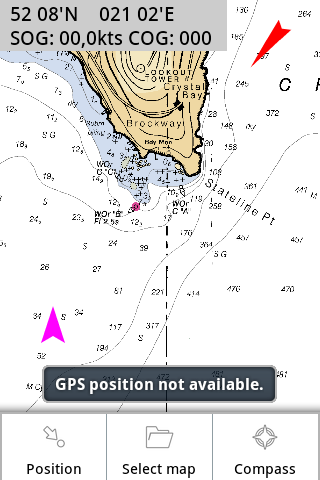
\includegraphics[scale=0.45]{screen1}
\end{center}
\end{frame}

\begin{frame}
\frametitle{Prezentacja}
\end{frame}

\subsection{Cechy}
\begin{frame}
\frametitle{Główne cechy}
\begin{itemize}
	\item {własny interpreter zdarzeń dotyku - komunikacja zdarzeniowa}
	\item {obsługa zdarzeń kompasu zależnie od położenia telefonu}
	\item {cykliczne sprawdzanie obecności sygnału GPS}
	\item {zarządzanie pamięcią}
	\item {pamiętanie ustawień}
\end{itemize}
\end{frame}

\section{Wnioski}
\subsection{Wrażenia}
\begin{frame}
\frametitle{Co było ciekawe?}
Co było ciekawe?
\begin{itemize}
	\item {obsługa czujników - kompas, dotyk, GPS}
	\item {projektowanie interfejsu}
	\item {obsługa mapy z odpowiednią dokładnością}
\end{itemize}
\vskip20pt
\pause
Co było nieciekawe / męczące?
\begin{itemize}
	\item {ograniczenia systemu Android - pamięć}
	\item {brak bibliotek (libbsb)}
	\item {API Androida}
	\item {ciężkie do znalezienia wskazówki jak tworzyć \textbf{dobry} kod}
\end{itemize}
\end{frame}

\subsection{Co jeszcze?}
\begin{frame}
\frametitle{Co jeszcze?}
\begin{itemize}
	\item {obsługa dużych map}
	\item {natywne wsparcie dla formatu BSB}
	\item {zintegrowana przeglądarka map}
	\item {...}
\end{itemize}
\end{frame}

\end{document}


